\hypertarget{1}{}

\chapter{Introduction}

\rhead{Introduction}
\lhead{Chapter 1}

\vspace{-1.6cm}

% Gray Line
\begingroup
\color{gray}
\par\noindent\rule{\textwidth}{0.4pt}
\endgroup

\noindent{This chapter presents the motivation, objectives, general methodology, and contributions of this dissertation, as well as the overall document structure.}

% ------------------------------> MOTIVATION

\section{Motivation}

Biomedical literature is the main medium that researchers use to share their findings, mainly in the form of articles, patents, and other types of written reports \citep{P99-1001}. A researcher working on a specific topic needs to be up-to-date with all developments regarding the work done on the same topic. However, the volume of textual information available widely surpasses the ability of analysis by a researcher even if restricting it to a domain-specific topic. Not only that, but the textual information available is usually in an unstructured or highly heterogeneous format. Thus, retrieving relevant information requires not only a considerable amount of manual effort but is also a time-consuming task. 

Scientific articles are the primary source of knowledge for biomedical entities and their relations. These entities include human phenotypes, genes, proteins, chemicals, diseases, and other biomedical entities inserted in specific domains. A comprehensive source for articles on this topic is the PubMed\footnote{\url{https://www.ncbi.nlm.nih.gov/pubmed/}} platform, combining over 29 million citations while providing access to their metadata. Processing this volume of information is only feasible by using text mining solutions.

Automatic methods for Information Extraction (IE) aim at obtaining useful information from large data sets \citep{REVIEW}. Text mining uses IE methods to process text documents. Text mining systems usually include Named-Entity Recognition (NER), Named-Entity Linking (NEL), and Relation Extraction (RE) tasks. NER consists of recognizing entities
mentioned in the text by identifying the offset of its first and last character. NEL consists of mapping the recognized entities to entries in a given knowledge base. RE consists of identifying relations between the entities mentioned in a given document. A detailed definition of these tasks will be provided in Section \hyperlink{2.2.1}{2.2.1}. Some of the commonly extracted biomedical relations are protein-protein interactions \citep{PROTEIN-PROTEIN}, drug-drug interactions \citep{BOLSTM} and disease-gene relationships \citep{DISEASE-GENE}.

RE can be performed by different methods, namely, by order of complexity, co-occurrence, pattern-based (manually or automatically created), rule-based (manually or automatically created), and machine learning (feature-based, kernel-based, multi-instance, and Recurrent Neural Networks (RNN)). Distantly supervised multi-instance learning uses a knowledge base of gold standard target relations (distant supervision) combined with a sparse multi-instance learning (sMIL) algorithm  \citep{Bunescu:2007:MIL:1273496.1273510} to perform RE. Distant supervision assumes that any sentence that mentions a pair of entities corresponding to a knowledge base entry is likely to describe a relation between those entities \citep{10.1371/journal.pone.0171929}. These candidate relations can be used to train a classifier using the multi-instance algorithm. More recently, deep learning techniques, such as RNN, have achieved outstanding results at various Natural Language Processing (NLP) tasks, among them RE. The success of deep learning for biomedical NLP is in part due to the development of word vector language models like Word2Vec \citep{Mikolov:2013:DRW:2999792.2999959}, and, more recently, ELMo \citep{DBLP:journals/corr/abs-1802-05365}, BERT \citep{BERT}, GPT \citep{Radford2018ImprovingLU}, Transformer-XL \citep{2019arXiv190102860D}, and GPT-2 \citep{gt2}. These models learn word vector representations also known as word embeddings that capture the syntactic and semantic word relationships. Long Short-Term Memory (LSTM) networks constitute a variant of artificial neural networks presented as an alternative to regular RNN \citep{Hochreiter:1997:LSM:1246443.1246450}. LSTM networks deal with more complex sentences, making them more fitting for biomedical literature. %To improve their results in a given domain, it is possible to integrate external sources of knowledge such as domain-specific ontologies.

The knowledge encoded in the various domain-specific ontologies, such as the Gene Ontology (GO) \citep{GO}, the Chemical Entities of Biological Interest (ChEBI) ontology \citep{CHEBI}, and the Human Phenotype Ontology (HPO) \citep{HPO} is deeply valuable for detection and classification of relations between different biomedical entities. Besides that these ontologies make available important characteristics about each entity, they also provide us with the underlying semantics of the relations between those entities, such as is-a relations. For example, \textit{neoplasm of the endocrine system} (HP:0100568), a phenotypic abnormality that describes a tumor (abnormal growth of tissue) of the endocrine system \textbf{is-a} \textit{abnormality of the endocrine system} (HP:0000818), and \textbf{is-a} \textit{neoplasm by anatomical site} (HP:0011793), which in turn \textbf{is-a} \textit{neoplasm} (HP:0002664) (Figure \ref{figure:1}). 

\begin{figure}[ht]
\captionsetup{font=small}
\centering
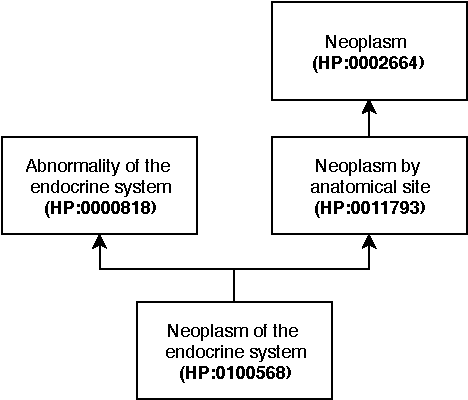
\includegraphics[width=10cm]{images/figure_1.pdf}
\fontsize{9}{10.8}\caption[HPO Ontology Excerpt]{An excerpt of the HPO ontology showing the first ancestors of \textit{neoplasm of the endocrine system}, using \textbf{is-a} relationships.}
\label{figure:1}
\end{figure}

The information provided by the ancestors is not expressed directly in the text and can support or disprove an identified relation. Ontologies are formally organized in machine-readable formats, facilitating their integration in relation extraction models. 

Using different sources of information, as additional data, to support automating searching for relations between biomedical concepts contributes to the development of pharmacogenomics, clinical trial screening, and adverse drug reaction identification \citep{10.1093/bib/bbx048}. Identifying new relations can help validate the results of recent research, and even propose new experimental hypotheses.

% ------------------------------> OBJECTIVES

\hypertarget{1.2}{\section{Objectives}}

The fundamental challenge of contemporary genetic analysis is correlating genes to their respective phenotypes. Existing systems that have the flexibility to be applied for the identification and extraction of human phenotype-gene relations, from biomedical literature, are scarce and limited. The main challenges that they face are the lack of annotated data sets; difficulties in the identification of phenotype entities, that are composed of multiple words, which makes name boundaries complex; and a scarcity of experts to perform curation of the identified relations. All of the aforementioned creates the need for automated corpora creation tools and the development of machine learning systems that can deal with the versatility of the gene and human phenotype entities and their relations, to better identify and extract them from text. Thus, the main goals of this work are:

\begin{enumerate}
\item{Create a large and versatile silver standard corpus of human phenotype-gene relations.}

\item{Develop a distantly supervised multi-instance learning module that combines a knowledge base for automatic extraction of human phenotype-gene relations (added to the IBRel system \citep{10.1371/journal.pone.0171929}).}

\item{Develop a deep learning module for automatic extraction of human phenotype-gene relations, taking advantage of domain-specific ontologies, like the Human Phenotype Ontology (HPO) and the Gene Ontology (added to the BO-LSTM system \citep{BOLSTM}).}
\end{enumerate}

First, the proposed pipeline should be able to generate a silver standard corpus based on articles dedicated to human phenotype-gene relations, using existing NER tools, and a gold standard relations knowledge base, provided by the HPO. Second, both machine learning systems (distantly supervised multi-instance learning, and deep learning) should be able to use the previous corpus to train a classifier and compare the classifications against a manually curated test-set.

The \textbf{hypothesis} of this dissertation is that information about human phenotype-gene relations can be efficiently extracted from biomedical literature using an automatically generated corpus, and machine learning techniques along with domain-specific ontologies.

% ------------------------------> METHODOLOGY

\section{Methodology}

The overall methods to accomplish the proposed objectives can be divided into three stages, one for each objective. The first stage is the creation of a silver standard human phenotype-gene relations corpus (generated in a fully automated manner) (Chapter \hyperlink{3}{3}), the second and third stages are the development of a distantly supervised multi-instance learning module that combines a knowledge base, and the development of a deep learning module that takes advantage of domain-specific ontologies, both for automatic extraction of human phenotype-gene relations (Chapter \hyperlink{4}{4}). 

To generate a silver standard for phenotype-gene relations, we need a pipeline that performs NER to recognize genes and human phenotype entities, and RE to extract and classify a relation between the identified human phenotype and gene entities. The first step is to gather abstracts using the PubMed API with manually defined keywords, namely, each gene name that participates in a relation (retrieved from a gold standard knowledge base of relations), \textit{homo sapiens}, and \textit{disease}. Then, the NER stage is performed using the Minimal Named-Entity Recognizer (MER) tool \citep{MER} to extract gene mentions, and the Identifying Human Phenotypes (IHP) tool \citep{IHP} to extract human phenotype mentions, from the abstracts. At last, using a gold standard relations knowledge base, provided by the HPO, the relations obtained by co-occurrence of the entities in the same sentence are marked \textit{Known} or \textit{Unknown}, and a subset (test-set) of the relations curated by domain experts. The \textit{Known} relations are in the knowledge base and the \textit{Unknown} relations are not yet identified or that do not exist.
The test-set was created by randomly selecting 260 relations to be reviewed by eight curators (50 relations each, with an overlap of 20 relations), all researchers working in the areas of Biology and Biochemistry.

While in the first stage a distant supervision approach is used to mark the relations with \textit{Known} or \textit{Unknown}, in the second stage the unlabeled silver standard corpus is going to be used to apply the distantly supervised multi-instance learning approach. These two distant supervision approaches differ in the way they are applied, as we are going to see in the following chapters.  

In the second stage, the goal is to use the corpus generated in the first stage unlabeled (annotated only with entity mentions) combined with a knowledge base (provided by the HPO), that provides examples for the relations we wanted to extract, to apply distantly supervised multi-instance learning. The best feature of this machine learning approach is the fact that it does not require the relations annotations, only the human phenotype and gene entities mentions, reducing the amount of manual effort necessary.

For the last stage, the main goal is to combine RNN (deep learning) algorithms with biological ontologies to improve the identification of human phenotype-gene relations in biomedical literature. Ontologies such as the HPO and the Gene Ontology provide a reliable representation of their respective domains and can be used as data representation layers to extract relations from text. The proposed system is going to represent each candidate pair as the sequence of the relations between the entities ancestors in their respective ontology and combine word embeddings and WordNet (generic English language ontology) to produce a model able to extract the \textit{Known} relations from text.

% ------------------------------> CONTRIBUTIONS

\hypertarget{1.4}{\section{Contributions}}

The main contribution of this dissertation was a feasible solution to identify and extract human phenotype-gene relations from text, that may be applied to other types of biomedical relations. This dissertation created the first corpus specific to human phenotype-gene relations, in an attainable and reproducible way, and two different system modules to extract these type of relations from highly heterogeneous text. Both the silver standard corpus and the developed modules evaluation was done with a test-set curated by domain experts. This section provides an overview of the contributions related to each of the objectives initially defined in Section \hyperlink{1.2}{1.2}. One contribution that did not corresponded to the initially defined goals was a book chapter presenting the base concepts for neural networks using ontologies for RE:

\begin{itemize}
    \item{\textbf{Book Chapter Submitted} \citep{book}: \textit{Using Neural Networks for Relation Extraction from Biomedical Literature for the book Artificial Neural Networks: Methods and Applications} (Diana Sousa, André Lamúrias, and Francisco M. Couto) in the Springer "Methods in Molecular Biology" series.}
\end{itemize}

% ----------------> OBJECTIVE 1

\subsection{Objective 1}

Chapter \hyperlink{3}{3} presents a pipeline to generate a silver standard human phenotype-gene relations corpus. The pipeline required the application of two NER tools and the availability of a list of gold standard relations. The evaluation of the corpus resorted to eight curators obtaining 87.01\% in precision with an inter-agreement of 87.58\%. The work developed for this objective resulted in one freely available silver standard corpus of human phenotype-gene relations\footnote{\url{https://github.com/lasigeBioTM/PGR}} and one paper accepted for the proceedings of an international conference (Core A):

\begin{itemize}
    \item{\textbf{Paper Accepted} \citep{DBLP:journals/corr/abs-1903-10728}: \textit{A Silver Standard Corpus of Human Phenotype-Gene Relations} (Diana Sousa, André Lamúrias, and Francisco M. Couto) in the Proceedings of the 2019 North American Chapter of the Association for Computational Linguistics.}
\end{itemize}

% ----------------> OBJECTIVE 2

\subsection{Objective 2}

Section \hyperlink{4.1.1}{4.1.1} presents a distantly supervised multi-instance learning module added to the IBRel system, to extract human phenotype-gene relations from text. The pipeline required a list of gold standard human phenotype-gene relations, the same as used in Chapter \hyperlink{3}{3}. The evaluation of the module resorted to the PGR test-set obtaining 73.48\% in F-measure. The work developed for this objective produced a high-performance distantly supervised multi-instance learning module that can effectively extract human phenotype-gene relations from text.

% ----------------> OBJECTIVE 3

\subsection{Objective 3}

Section \hyperlink{4.1.2}{4.1.2} presents a deep learning module added to the BO-LSTM system, able to extract human phenotype-gene relations from text. The pipeline required the ontologies available for both type of entities (HPO and Gene Ontology). These were added to the module as data representation layers to feed the deep learning model. The evaluation of the module resorted to the PGR test-set obtaining 55.00\% in F-measure. The work developed for this objective resulted in one journal publication (Q1 Scimago):

\begin{itemize}
    \item{\textbf{Paper Published} \citep{BOLSTM}: \textit{BO-LSTM: Classifying Relations Via Long
    Short-term Memory Networks Along Biomedical Ontologies} (André Lamúrias, \textbf{Diana Sousa}, Luka A. Clarke, and Francisco M. Couto) in BMC Bioinformatics.}
\end{itemize}

% ------------------------------> DOCUMENT STRUCTURE

\section{Document Structure}

Additionally to the present introductory chapter, this document is structured in four chapters as follows:

\begin{itemize}
   \item \textbf{Chapter \hyperlink{2}{2}} (Related Work) introduces the basic concepts and resources that support RE techniques, namely, Natural Language Processing (NLP), text mining primary tasks, initial approaches for RE, distant supervision for RE, neural networks for RE, and evaluation measures.
   \item \textbf{Chapter \hyperlink{3}{3}} (A Silver Standard Corpus of Phenotype-Gene Relations) presents the work developed to create a silver standard corpus of human phenotype-gene relations, including methods, evaluation, results and discussion.
   \item \textbf{Chapter \hyperlink{4}{4}} (Extracting Phenotype-Gene Relations) presents the system modules developed (distantly supervised multi-instance and deep learning modules) to accommodate human phenotype-gene RE, with methods, evaluation, results and discussion, for each module, and a detailed comparison between the two.
   \item \textbf{Chapter \hyperlink{5}{5}} (Conclusion) discusses the main conclusions of this work, and indicates some directions for future work.
\end{itemize}